% ***********************************************************************************
% Pure LaTeX part to be inserted in a document (be careful of depencies of packages & commands
% Prepared by Qingan Zhao under the supervision of Arnaud de La Fortelle
% Fall 2017
% Example of solving the 2D heat diffusion subsection of the modeling part part
% ***********************************************************************************

\subgroup{2}{Qingan Zhao}

\paragraph{Description}
Now consider a retangular plane (length: a; width: b) with 2 boundaries that have no heat transfer (i.e., $T(x, 0)=f(x);\ T(x, b)=g(x)$). The other two boundaries have fixed temperature ($T(0, y)=T(a, y)=0$). We would like to solve the PDE under the stationary state (i.e., $\ud T/\ud t=0$). The diagram of the system is shown in Figure~\ref{heatSolSystem.fig}.
\begin{figure}[htb]
	\centering
	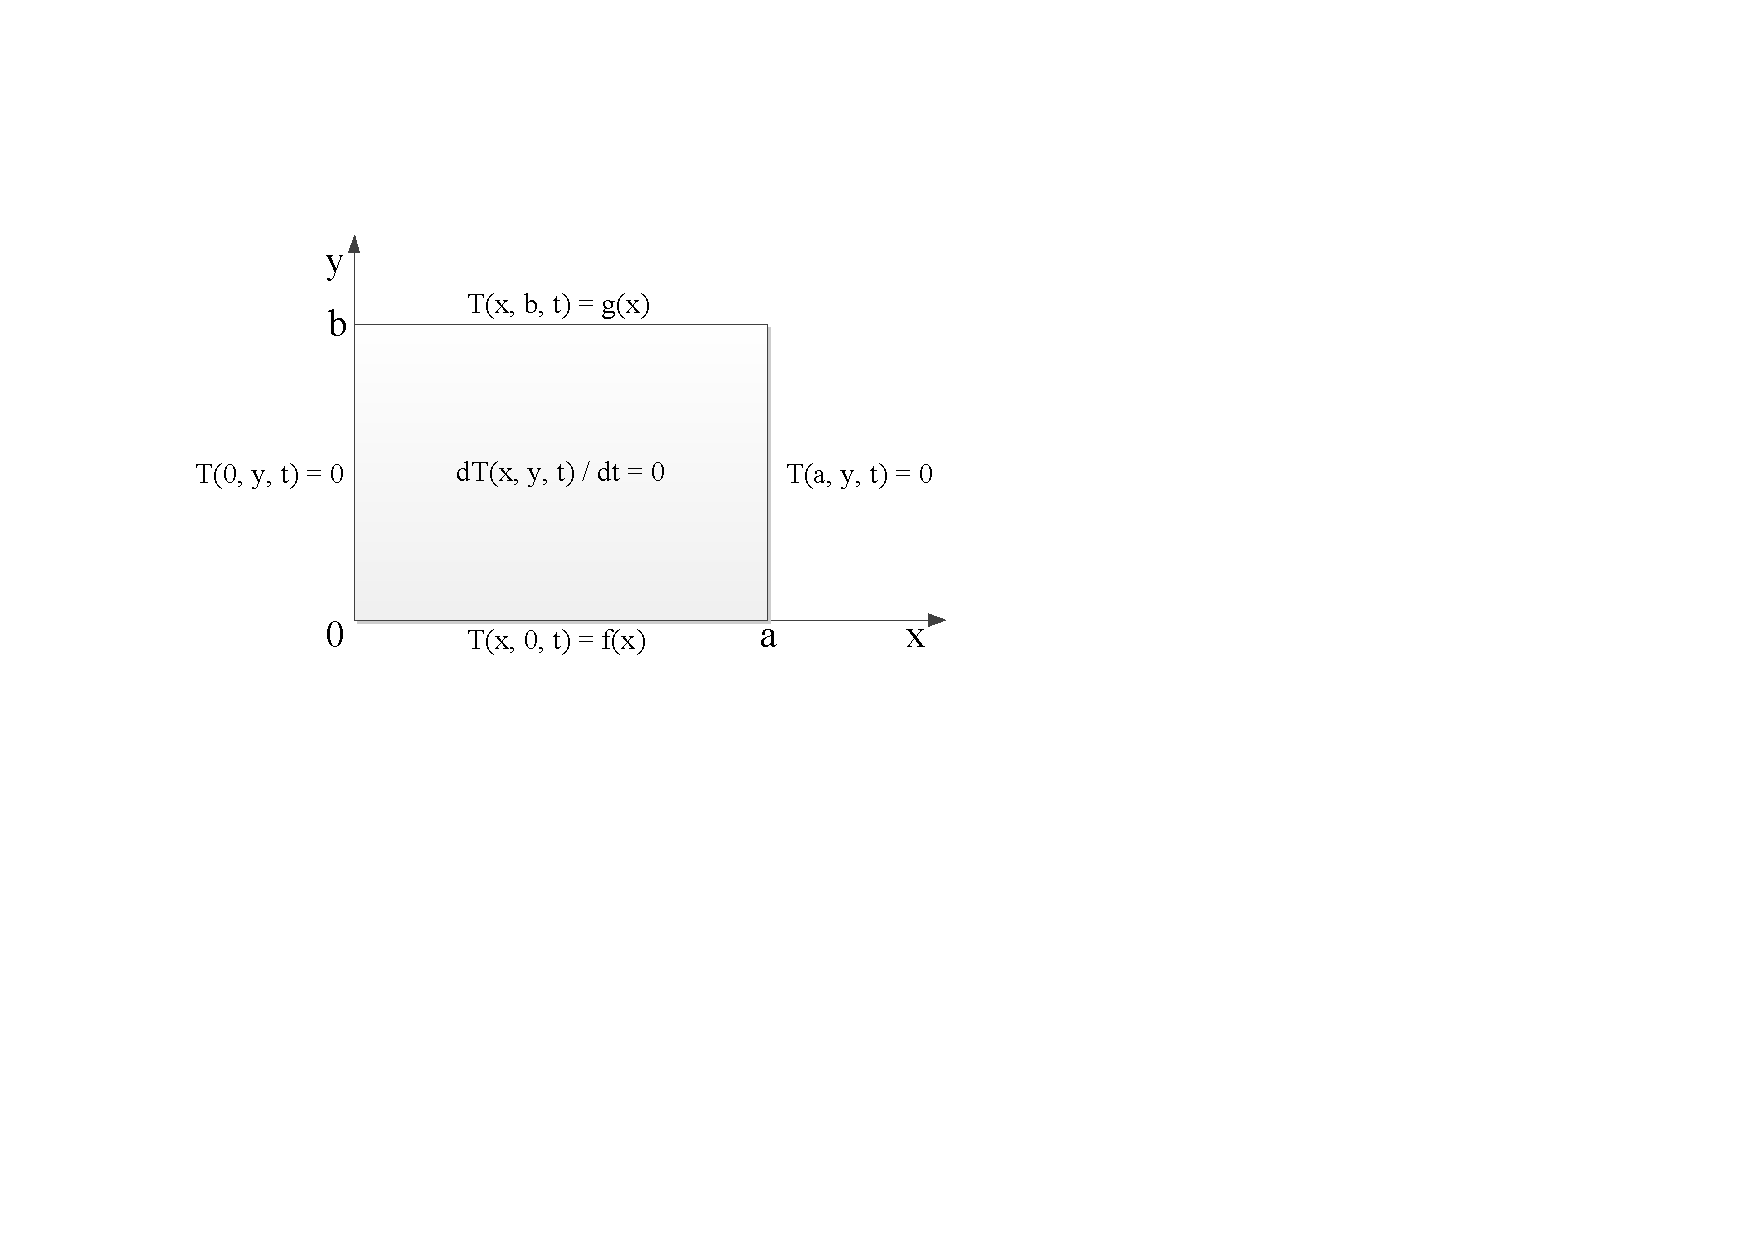
\includegraphics[width=10cm]{2dHeatSolDescription.pdf}       
	\caption{System description of the example}\label{heatSolSystem.fig}
\end{figure}

\paragraph{PDE and boundary conditions}
From Section 2.2.2 we have already known that the 2D heat equation is:
\begin{equation}
\frac{\partial T}{\partial t}=a^2\left(\frac{\partial ^2 T}{\partial x^2}+\frac{\partial ^2 T}{\partial y^2}\right)\ \ \ \ where\ a=\sqrt{\frac{k}{c\rho}}
\end{equation}


The boundary conditions of this problem are as follows:

\begin{equation}\label{2DHeatBound1.eq}
T(x,0,t)=f(x)
\end{equation}
\begin{equation}\label{2DHeatBound2.eq}
T(x,b,t)=g(x)
\end{equation}
\begin{equation}\label{2DHeatBound3.eq}
T(0, y, t)=0
\end{equation}
\begin{equation}\label{2DHeatBound4.eq}
T(a, y, t)=0
\end{equation}
\begin{equation}
\frac{\ud T}{\ud t}=0
\end{equation}

\paragraph{Solution}
Since the system is under the stationary state ($\ud T/\ud t=0$), $T(x,y,t)$ can be expressed as $T(x,y)$, and the PDE can be written as:
\begin{equation}
\frac{\partial^2T}{\partial x^2}+\frac{\partial^2T}{\partial y^2}=0
\end{equation}

We could sperate the variables by express $T(x,y)$ as $X(x)Y(y)$. Then the PDE can be written as:
\begin{equation}
X''(x)Y(y)+X(x)Y''(y)=0
\end{equation}

Since $X(x)Y(y)$ is not identically zero, divide both sides by $X(x)Y(y)$ gives:
\begin{equation}
\frac{X"(x)}{X(x)}+\frac{Y"(y)}{Y(y)}=0
\end{equation}

Since the two parts of the left side are independent, the following equations can be drawn ($\lambda$ is a constant):
\begin{align}
X"(x)+\lambda X(x)=0\\
Y"(y)-\lambda Y(y)=0
\end{align}

Moreover, the boundary conditions Equations~(\ref{2DHeatBound3.eq})-(\ref{2DHeatBound4.eq}) give:
\begin{align}
X(0)Y(y)=0\\
X(a)Y(y)=0
\end{align}

Since $Y(y)$ is not identically zero, we can obtain the following:
\begin{align}
X(0)=0\\
X(a)=0
\end{align}

Hence, the problem becomes solving two indenpendent ordinary differential equations. We know that only when $\lambda=\frac{n^2\pi^2}{a^2}\ (n=1,2,3,...)$, the problem has the following solution:
\begin{equation}
X_n(x)=\sqrt{\frac{2}{a}}sin\frac{n\pi x}{a}
\end{equation}
\begin{equation}
Y_n(y)=a_ne^{\frac{n\pi}{a}y}+b_n^{-\frac{n\pi}{a}y}
\end{equation}

Hence, the solution can be expressed as:
\begin{equation}
T(x,y)=\sqrt{\frac{2}{a}}\sum_{n=1}^{\infty}(a_ne^{\frac{n\pi}{a}y}+b_n^{-\frac{n\pi}{a}y})sin\frac{n\pi x}{a}
\end{equation}

Given the other two boundary conditions Equations~(\ref{2DHeatBound1.eq})-(\ref{2DHeatBound2.eq}), $a_n$ and $b_n$ can be solved using the following 2 equations:
\begin{equation}
a_n+b_n=\sqrt{\frac{2}{a}}\int_{0}^{a}f(x)sin\frac{n\pi}{a}xdx
\end{equation}
\begin{equation}
a_ne^{\frac{n\pi}{a}b}+b_ne^{-\frac{n\pi}{a}b}=\sqrt{\frac{2}{a}}\int_{0}^{a}g(x)sin\frac{n\pi}{a}xdx
\end{equation}

Thus, the analytical solution of this problem is solved.















